\documentclass[a4paper]{article}
\usepackage{graphicx}
\usepackage{amsmath,amssymb}
\usepackage{hyperref}
\usepackage{minted}
\usepackage{multirow}
\usepackage{float}

\title{Genus}
\date{}

\begin{document}
    \maketitle
    ``Genus`` is auf Englisch ``Gender``
    
\n    \\section{Gender recognition rules}\n    The safest method is to learn every noun together with its article. The following rules help predict the gender, but some have exceptions.\n\n    \\subsection{Substantivierung}\n    \\textbf{Substantivierung} (also: Nominalisierung) means using another word class as a noun.\n\n    \\paragraph{Substantivierung von Verben}\n    A substantivized infinitive (\\textbf{substantivierter Infinitiv}) is always \\textbf{neutral (das)} and is capitalized:\n    \\textit{das Lernen, das Essen, das Schwimmen, das Spazierengehen}.\n\n    \\paragraph{Substantivierung von Adjektiven}\n    Substantivized adjectives do not have one fixed gender. Their gender depends on the person or thing they refer to, and they keep adjective declension:\n    \\textit{der Deutsche, die Deutsche, das Gute, die Reichen}.\n\n    \\subsection{Gender from suffixes}\n    \\textbf{Usually feminine (die):} -ung, -heit, -keit, -schaft, -ei/-erei, -ion, -tät, -ik, -ur; and -in for female persons.\n    Examples: \\textit{die Wohnung, die Freiheit, die Möglichkeit, die Gesellschaft, die Bäckerei, die Situation, die Universität, die Musik, die Natur, die Studentin}.\n\n    \\textbf{Usually masculine (der):} -ling, -ismus, -ist, -or; many agent/person nouns in -er.\n    Examples: \\textit{der Schmetterling, der Kapitalismus, der Polizist, der Motor, der Lehrer}.\n\n    \\textbf{Usually neutral (das):} -chen and -lein (always neutral); -ment, -um and many nouns in -ma; many borrowed nouns in -o.\n    Examples: \\textit{das Mädchen, das Büchlein, das Instrument, das Zentrum, das Thema, das Auto}.\n\n    \\subsection{Gender from meaning}\n    \\textbf{Usually masculine:} male persons/professions; days, months and seasons; cardinal directions; many weather phenomena.\n    Examples: \\textit{der Vater, der Lehrer, der Montag, der September, der Sommer, der Norden, der Wind, der Regen}.\n\n    \\textbf{Usually feminine:} female persons/professions; many names of trees and flowers.\n    Examples: \\textit{die Mutter, die Lehrerin, die Eiche, die Rose}. Exceptions exist, e.g. \\textit{der Ahorn}.\n\n    \\textbf{Usually neutral:} young humans/animals; metals and chemical elements (with exceptions).\n    Examples: \\textit{das Kind, das Baby, das Kalb, das Gold, das Eisen}.\n\n    \\subsection{Compound nouns (Komposita)}\n    In a compound noun, the \\textbf{last component determines the gender}. This is one of the most reliable rules:\n    \\textit{die Arbeit + der Platz = der Arbeitsplatz}; \\textit{das Haus + die Tür = die Haustür}; \\textit{die Sprache + das Buch = das Sprachbuch}.\n\n    \\subsection{Important cautions}\n    \\begin{itemize}\n      \\item Natural sex does not always determine grammatical gender: \\textit{das Mädchen} is neutral because -chen is neutral.\n      \\item Similar meanings can have different genders: \\textit{der Wagen, das Auto, die Limousine}.\n      \\item A suffix rule applies only when the ending really functions as that suffix.\n      \\item If no reliable rule applies, learn the article with the noun: not just \\textit{Tisch}, but \\textbf{der Tisch}.\n    \\end{itemize}\n\n    \\subsection{Quick strategy}\n    \\begin{enumerate}\n      \\item Substantivized infinitive? $\\rightarrow$ \\textbf{das}.\n      \\item Compound noun? $\\rightarrow$ gender of the last component.\n      \\item Strong gender suffix? Use it.\n      \\item Clear semantic group? Use that clue.\n      \\item Otherwise, check and memorize the article with the noun.\n    \\end{enumerate}\n
    \begin{figure}[H]
        \centering
        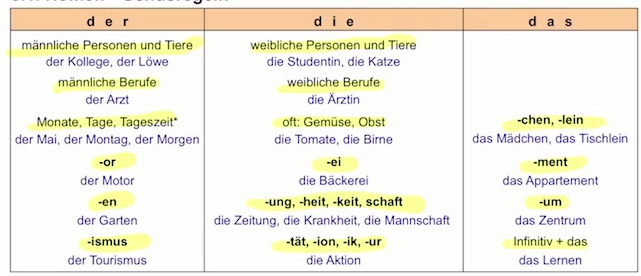
\includegraphics[width=0.9\textwidth]{genus.png}
    \end{figure}
    
    \begin{figure}[H]
        \centering
        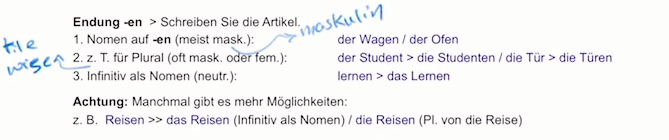
\includegraphics[width=0.9\textwidth]{genus_exception.png}
    \end{figure}
    % \bibliographystyle{plain}
    % \bibliography{/home/donkarlo/Dropbox/repo/shared_research/refs/refs}
\end{document}